\documentclass{beamer}
    \usepackage[brazil]{babel}
    \usepackage[utf8]{inputenc} 

    \makeatletter
    \def\verbatim{\tiny\@verbatim \frenchspacing\@vobeyspaces \@xverbatim}
    \makeatother
       
    \pgfdeclareimage[height=1.2cm]{logo}{./imagens/logoUdescFinal}
    \logo{\pgfuseimage{logo}}
    
    \pgfdeclareimage[height=6cm]{duvidas}{./imagens/ponto1}

    \usetheme{Berkeley}

  
%%% Numerar slides
%%% Ref: https://tex.stackexchange.com/a/145899
%%% https://tex.stackexchange.com/questions/145829/slide-number-in-beamer-berkeley-header
\makeatletter
\setbeamertemplate{frametitle}{%
    \nointerlineskip%
    \vskip-\beamer@headheight%
    \vbox to \beamer@headheight{%
      \vfil
      \leftskip=-\beamer@leftmargin%
      \advance\leftskip by0.3cm%
      \rightskip=-\beamer@rightmargin%
      \advance\rightskip by0.3cm plus1fil%
      {\usebeamercolor[fg]{frametitle}
          \usebeamerfont{frametitle}\insertframetitle\hfill\insertframenumber\par}% added number
      {\usebeamercolor[fg]{framesubtitle}
           \usebeamerfont{framesubtitle}\insertframesubtitle\par}%
      \vbox{}%
      \vskip-1em%
      \vfil
    }%
  }
\makeatother

    
    \title{Trabalho Complementar 1}
    \author{Gustavo José Neves da Silva}

    \date{}
    
    
    \begin{document}
    
    \begin{frame}
      \titlepage
    \end{frame}
    
  %  Fazer uma apresentação de 10 minutos para cada trabalho:
  %  Qual foi o problema?
  %  Qual o objetivo?
  %  O que fez o TCC?
  %  Que recursos/técnicas usou?
  %  Que resultados obteve?
  %  Que concluiu com o TCC?
  %  Quais sub-áreas está relacionado e PORQUE.
\section{Trabalho}
\begin{frame}[fragile]
    \frametitle{Qual foi o problema?}
    A reconstrução tridimensional por meio da interpolação de curvas com mudança topológica pode gerar diferentes modelos geométricos.

\end{frame}

\begin{frame}[fragile]
  \frametitle{Qual o objetivo?}
  Obter uma solução algorítmica a fim de estabelecer critérios para a interpolação linear quando ocorrer mudança topológica entre as seções.
  \begin{figure}
    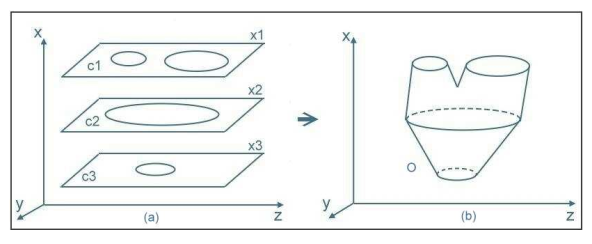
\includegraphics[height=4cm]{./imagens/image3721}
    \caption{"Mudança Topológica, (ANZOLLIN, 2006)"}
  \end{figure}
\end{frame}

\begin{frame}[fragile]
  \frametitle{O que fez o TCC?}
  Propõe o algoritmo Delta-Connection.
  %, o qual dá enfase a etapa de correspondência, não trata com precisão cada local de bifurcação e obtêm um resultado direto, porém impreciso da etapa de geração de malha.

\end{frame}


\begin{frame}[fragile]
  \frametitle{Recursos/técnicas utilizadas}
  \begin{itemize}
    \item Interpolação de curvas
    \item VRML
    \item XML
    \item Representação poligonal/vetorial
    \item Bounding Box(cálculo do centróide)
    \item Boundary Representation(B-rep)
    \item Triangulação
  \end{itemize}
\end{frame}

\begin{frame}[fragile]
  \frametitle{Resultados obtidos}
  Foi apresentada uma solução para o problema de interpolação de curvas com mudança topológica baseada em abordagens heurísticas de reconstrução tridimensional
  %, tendo como critérios de eficiência a rapidez e simplicidade no cálculo das etapas de reconstrução.

\end{frame}

\begin{frame}[fragile]
  \frametitle{Conclusões do trabalho}
  Com base nos resultados apresentados a partir dos testes, o trabalho alcançou seus objetivos.
\end{frame}


\begin{frame}[fragile]
  \frametitle{Sub-áreas relacionadas}
  \begin{itemize}
    \item Visualização Científica
    \item Reconstrução tridimensional
    \item Representação de canais
    \item Modelagem Geométrica
  \end{itemize}

\end{frame}


\section{Referências}
\begin{frame}[fragile]
    \frametitle{Referências}
    \begin{footnotesize}
        \begin{verbatim}
          ANZOLLIN, Guilherme Rossetti; HOUNSELL, Marcelo da Silva.
          Interpolação de curvas com mudança topológica. 2006. 83 f.
          Trabalho de conclusão de curso (Graduação)
          Universidade do Estado de Santa Catarina, Curso de Ciência da Computação, 2006.
        \end{verbatim}
    \end{footnotesize}
\end{frame}
    
    
\section{Dúvidas}
\begin{frame}[fragile]
    \frametitle{Perguntas}
        \begin{center}
            \pgfuseimage{duvidas}
        \end{center}

\end{frame}
    
\end{document}
    
